\section{Full state, basic and passivity-based feedback controllers} 
\label{sec:Full_state_feedback_controllers}

From the full dynamic model of the exoskeleton, a novel  full state feedback control law   was  derived and implemented. This control law is  identified in the following with the acronym JTFC1  and  explained in subsection \ref{subsec:JTFC1}.
To implement the control, the state of the system and, more in particular, the joint torque was estimated through a Kalman Filter described in  subsection \ref{subsec:kalmanTorque}.
To evaluate the performance of  the proposed full state feedback control,  two other torque controls inspired to existing joint torque controls available in literature have been implemented, identified respectively with the acronyms JTFC2 and JTFC3.
% We searched for torque controls designed for joint torque-based robots with a joint structure similar to the Rehab-Exos one.
\par The JTFC2, presented in subsection \ref{subsec:JTFC2}, is based on a  torque control   for  single joint based on torque sensor first  introduced by Hashimoto \cite{hashimoto1998experimental}. In order to compare the basic torque control with our full state feedback control, the Hashimoto formulation was extended and generalized to a multi-dof case. 
\par The JTFC3, reported in subsection \ref{subsec:JTFC3}, was inspired to the passivity-based control law \cite{kugi2008passivity}
implemented for the DLR Light Weight Robot III (LWR III)   that guarantees the passivity of the controlled system. The DLR LWR III shows a joint design compatible with the Rehab-Exos one, since both systems make use of the joint torque sensor to estimate the interaction torques/forces with the environment/human.


%%%%%%%%%%%%%%%%%%%%%%%%%%%%%%%%%%%%%%%%%%%%%%%%%%%%%%%%%%%%%%%%%%%%%%%%%%%%%%%%%%%%%%%%%%%%%%%%%%%%%%%%%%%%%%%%%%%%
%%%%%%%%%%%%%%%%%%%%%%%%%%%%%%%%%%%%%%%%%%%%%%%%%%%%%%%%%%%%%%%%%%%%%%%%%%%%%%%%%%%%%%%%%%%%%%%%%%%%%%%%%%%%%%%%%%%%
\subsection{An optimal observer for estimation of joint torque}\label{subsec:kalmanTorque}
Since the correct state estimation  is essential for the design of a full-state feedback joint-torque controller, the knowledge of the interaction torques between the human arm and the exoskeleton are required for  torque control implementation. The joint torque sensor provides a raw measurement $\tau_{s,i}$ that can be used together with the measured joint position $\theta_{m,i}$ to filter the sensed torque and to estimate the full system state, given by $[\tau_{s,i},\ \dot{\tau}_{s,i},\ \theta_{m,i},\ \dot{\theta}_{m,i},\ \tau_{d,i},\ \tau_{l,i}]$, where $\vects{\tau_l}=\vectm{J}^T \vects{F_l}$. 
Thus, a full-state Kalman filter has been designed to clean out both  $\theta_{m,i}$ from quantization noise $w_{\theta,i}$ and $\tau_{s,i}$ from measurement noise $w_{\tau,i}$, as well as to estimate the remaining variables.
%
\par 
Following \cite{vertechy2012interaction}, the dynamics of the two state components $\tau_{d,i}$ and $\tau_{l,i}$ can be modeled as two distinct Wiener processes (i.e. as two distinct non-stationary random processes) $\dot{\tau}_{d,i}=v_{d,i}$ and $\dot{\tau}_{l,i}=v_{l,i}$. Starting from \DIFdelbegin \DIFdel{equations (\ref{eq:dynamics_eq1},}\DIFdelend \DIFaddbegin \DIFadd{equation (}\DIFaddend \ref{eq:dynamics_eq2}) the following meta-system can be derived:
%DIF < 
%DIF > \ref{eq:dynamics_eq1},


%%%%%%DA VERIFICARE COSA SUCCESSO

\begin{equation}
\left \{
\begin{aligned}
\vects{\dot{\tau}_i} &=\vectm{A_i}\vects{\tau_i}+\vectm{B_i}\vects{\tau_{m,i}}+\vectmm{\Gamma}\vects{v_i} \\
		\vects{y_i} &=\vectm{C}\vects{\tau_i}+\vects{w_i}
		\end{aligned}
		\right .
		\label{eq:metasystem}
		\end{equation}
		%
		where $\vects{\tau_i}^T=[ \dot{\tau}_{s,i}\ \tau_{s,i}\ \dot{\theta}_{m,i}\ \theta_{m,i}\  \tau_{l,i} \tau_{d,i}\ ]$ is the meta-state vector, $\vects{v_i}^T=[ v_{l,i}\ v_{d,i} ]$ is the vector of process noises with variances $V_{l,i}$ and $V_{d,i}$, $\vects{w_i}^T=[ w_{\tau,i}\ w_{\theta,i} ]$ is the vector of measurement noises with variances $W_{l,i}$ and $W_{d,i}$, whereas:
		%
		\begin{equation}
		\begin{aligned}
		\vectm{A_i}=\mat{ \frac{-c_{t,i}}{J_i}  & \frac{-k_{t,i}}{J_i}& \frac{k_{t,i}b_{m,i}}{J_{m,i}} & 0 & \frac{ k_{t,i}}{J_{l,i}} &  \frac{-k_{t,i}}{J_{m,i}} \\
			1 & 0 & 0 & 0 & 0 & 0\\
			\frac{c_{t,i}}{  k_{t,i} J_{m,i} }&  \frac{1}{J_{m,i}} &  \frac{ -b_{m,i}}{J_{m,i}} & 0 & 0 &  \frac{1}{J_{m,i}}\\
			0 & 0 & 1 & 0 & 0 & 0\\
			0 & 0 & 0 & 0 & 0 & 0\\
			0 & 0 & 0 & 0 & 0 & 0} \\
		\vectm{B_i}=\vectlong{ \frac{ -k_{t,i}}{J_{m,i}} \\ 0 \\ \frac{1}{J_{m,i}} \\ 0 \\ 0 \\ 0}  \quad
		\vectmm{\Gamma}=\mat{ 0 & 0 \\ 0 & 0 \\ 0 & 0 \\ 0 & 0 \\ 1 & 0 \\ 0 & 1} \quad
		\vectm{C}=\mat{0 & 0 \\  1 & 0 \\  0 & 0  \\
			0 & 1 \\  0 & 0 \\ 0 & 0 } 
		\end{aligned}
		\label{stateobserver}
		\end{equation}
		%%%%%%%%%%%%%%%%%%%%%%%%%%%%%%%%%%%%%%%%%%%%%%%%%%%%%%%%%%%%%%%%%%%%%%%%%%%%%%%%%%%%%%%%%%%%%%%%%%%%%%%%%%%%%%%%%%%%
		%%%%%%%%%%%%%%%%%%%%%%%%%%%%%%%%%%%%%%%%%%%%%%%%%%%%%%%%%%%%%%%%%%%%%%%%%%%%%%%%%%%%%%%%%%%%%%%%%%%%%%%%%%%%%%%%%%%%



	\subsection{A full state feedback controller (JTFC1)} \label{subsec:JTFC1}

	The proposed control law is based on the full state obtained from the state  observer described by (\ref{eq:metasystem})  (\ref{stateobserver}), where the input control \DIFdelbegin \DIFdel{$\vects{u}$ }\DIFdelend \DIFaddbegin \DIFadd{$\vect{u}$ }\DIFaddend is splitted up into one term \DIFdelbegin \DIFdel{$\vects{u_f}$}\DIFdelend \DIFaddbegin \DIFadd{$\vect{u_f}$}\DIFaddend , which implement control force behavior, and another term $\vects{u_g}$, which acts as a gravity compensation

	\begin{equation}
	\label{generic_control_law1}
	\begin{aligned}
	\DIFdelbegin %DIFDELCMD < \vects{u} %%%
\DIFdelend \DIFaddbegin \vect{u} \DIFaddend &= \DIFdelbegin %DIFDELCMD < \vects{u_f} %%%
\DIFdelend \DIFaddbegin \vect{u_f} \DIFaddend + \DIFdelbegin %DIFDELCMD < \vects{u_g}
%DIFDELCMD < 	%%%
\DIFdelend \DIFaddbegin \vect{u_g}
	\DIFaddend \end{aligned}
	\end{equation}

The two above terms are expressed as:


\hl{SUBMITTED VERSION}

	
	\setlength{\arraycolsep}{0.0em}
	
	\begin{IEEEeqnarray}{ll}
			\DIFdelbegin %DIFDELCMD < \label{eq:JTCF1_control_law_a}
	\vects{u_g} &= \vects{G}(\vectm{D}\vects{\hat{\theta}_m}) \\
	\vects{u_fg} &  =- \vectm{J_m} \vectm{K_t}^{-1} \vects{\ddot{\tau}_s^D} + \vectm{B_m} \vectm{D}\vects{\dohat{\theta}_m} + \vectm{J_m} \overline{\vectm{M}^{-1}}  \vectm{J^T} \vects{\hat{F}_l} \nonumber  \\
	&{-}\:\vects{\hat{\tau}_d} - {\vectm{J}_i^{-1}} \vectm{J_m} \vects{\tau_s^D} + \vectm{K_p} \vects{e} + \vectm{K_dJ_m} \vects{\dot{e}}	
	\label{eq:JTCF1_control_law_b}
	\end{IEEEeqnarray}



\hl{REVISED}



\setlength{\arraycolsep}{0.0em}

\begin{IEEEeqnarray}{ll}
\label{eq:JTCF1_control_law_uf_simple}
\vect{u_g} &= \vect{G}(\vectm{D}\vects{\hat{\upthetau}_m}) \\
\vect{u_f} &=  -\overbrace{\colorboxed{green}{\vectm{I^{-1}_i} \vectm{I_m} \vects{\uptau^D_s}}}\DIFadd{^{\text{desired torque}}
			- }\overbrace{\colorboxed{red}{\vectm{I_m} \vectm{K^{-1}_t} (\vects{\ddot{\uptau}_s^D}- \vectm{K_d} \vect{\dot{e}} -  \vectm{K_p} \vect{e}  )}}\DIFadd{^{\text{state feedback}} + 	\nonumber \\
			&     +
\underbrace{\colorboxed{blue}{ (\vectm{I_m} \overline{\vectm{M}^{-1}}  \vectm{J^T} \vects{\hat{F}_l}+ \vectm{B_m} \vectm{D}\vects{\dot{\uptheta}_m} {-}\:\vects{\hat{\uptau}_d} ) }}\DIFadd{_{\text{unmodeled dynamics compensation}}
			}\DIFaddend \label{eq:JTCF1_control_law_b}
		\end{IEEEeqnarray}




where  \DIFdelbegin \DIFdel{$\vects{e}=\vects{\tau_s}-\vects{\tau_s^D}$ }\DIFdelend \DIFaddbegin \DIFadd{$\vect{e}=\vects{\uptau_s}-\vects{\uptau_s^D}$ }\DIFaddend is the error on sensor torque, given the desired sensor torque  \DIFdelbegin \DIFdel{$\vects{\tau_s^D}$}\DIFdelend \DIFaddbegin \DIFadd{$\vects{\uptau_s^D}$}\DIFaddend .
	Let us assume moreover that
	\DIFdelbegin \DIFdel{$\vects{\dot{\tau}^D=0}$ and  $\vects{\ddot{\tau}^D=0}$,
	so that 
	$\vects{\dot{e}}=\vects{\dot{\tau}_s}$ and $\vects{\ddot{e}}=\vects{\ddot{\tau}_s}$ the expression }%DIFDELCMD < \eqref{eq:JTCF1_control_law_b} %%%
\DIFdel{of $\vects{u_f}$ can be rewritten as
	}\DIFdelend 






%DIF > 	 the expression \eqref{eq:JTCF1_control_law_b} of $\vects{u_f}$ can be rewritten as
%DIF > 	
%DIF > 	\footnotesize
%DIF >DELCMD < 	\setlength{\arraycolsep}{0.0em}
%DIF >DELCMD < 	\begin{IEEEeqnarray}{l}
%DIF >DELCMD < 	\label{eq:JTCF1_control_law_uf_simple}
%DIF >DELCMD < 	\vects{u_f} = \: \vectm{B_m}   \vectm{D}\vects{\dot{\uptheta}_m} +  \vectm{IJ_m} \overline{\vectm{M}^{-1}} \vectm{J^T} \vects{\hat{F}_l} - {\vectm{IJ_i^{-1}}} \vectm{IJ_m} \vects{\uptau_s^D}  {-}\:\vects{\hat{\uptau}_d} + \vectm{K_p} \vects{e} + \vectm{K_d} \vects{\dot{e}}
%DIF >DELCMD < 	\end{IEEEeqnarray}
%DIF >DELCMD < 	\normalsize
%DIF >DELCMD < 	\setlength{\arraycolsep}{5pt}
\DIFaddbegin 

\DIFaddend The modified dynamics with the control laws  (\ref{generic_control_law1}), (\ref{eq:JTCF1_control_law_a}) and (\DIFdelbegin \DIFdel{\ref{eq:JTCF1_control_law_uf_simple}}\DIFdelend \DIFaddbegin \DIFadd{\ref{eq:JTCF1_control_law_b}}\DIFaddend ), leads to a stable error dynamics equations:

	\DIFdelbegin \begin{eqnarray*}\DIFdel{
		\vects{\ddot{\theta}_m} }&\DIFdel{= \vects{\ddot{\theta}_j} -\vectm{K_t^{-1}} \vects{\ddot{e}}
	}\\
	\DIFdel{\vects{0} }& \DIFdel{= \vects{\ddot{e}} + ( \vectm{C_t} \vectm{J_i^{-1}} + \vectm{K_d} \vectm{K_t}  \vectm{J_m^{-1}})\vects{\dot{e}}+ ( \vectm{K_t} \vectm{J_i^{-1}}  + \vectm{K_p}  \vectm{K_t}  \vectm{J_m^{-1}})\vects{e}
	}\end{eqnarray*}
	%DIFAUXCMD
	\DIFdelend \DIFaddbegin \begin{equation}\DIFadd{
		%	\vects{\ddot{\uptheta}_m} &= \vectm{D}^{-1} (\vects{\ddot{\uptheta}} -\vectm{K_t^{-1}} \vect{\ddot{e}})
		%DIF > \\
		\vects{0}  = \vect{\ddot{e}} + ( \vectm{C_t} \vectm{I_i^{-1}} + \vectm{K_d} )\vect{\dot{e}}+ ( \vectm{K_t} \vectm{I_i^{-1}}  + \vectm{K_p}   )\vect{e}
	}\end{equation}
	\DIFaddend 
	
	The convergence of error $\vects{e}$ to zero can so be adjusted by choosing the proportional and derivative gains $\vectm{K_p}$ and $\vectm{K_d}$, to obtain the desired dynamic response.


	
	
%	\DIFaddbegin \DIFadd{Based on the above, from the double derivation of }\eqref{eq:taus}\DIFadd{, we obtain the dynamics
%	}\begin{equation}\DIFadd{ 
%	\vects{\ddot{\uptheta}_m} = \vectm{D}^{-1} (\vects{\ddot{\uptheta}} -\vectm{K_t^{-1}} \vect{\ddot{e}}) \label{eq:taus_deriv} 
%	}\end{equation}	
%
%	
%	\DIFaddend \par Figure \ref{fig:full state} reports the schema of the proposed full state feedback control that takes into account the dynamic compensation contributes. Note that the torque sensor reads \DIFdelbegin \DIFdel{$\tau_{s,i}$ }\DIFdelend \DIFaddbegin \DIFadd{$\uptau_{s,i}$ }\DIFaddend and the commanded motor torques  \DIFdelbegin \DIFdel{$\tau_{m,i}$ }\DIFdelend \DIFaddbegin \DIFadd{$\uptau_{m,i}$ }\DIFaddend are net of the gravity compensation term $u_g$.





\begin{figure}[]
		\centering
	\DIFdelbeginFL %DIFDELCMD < 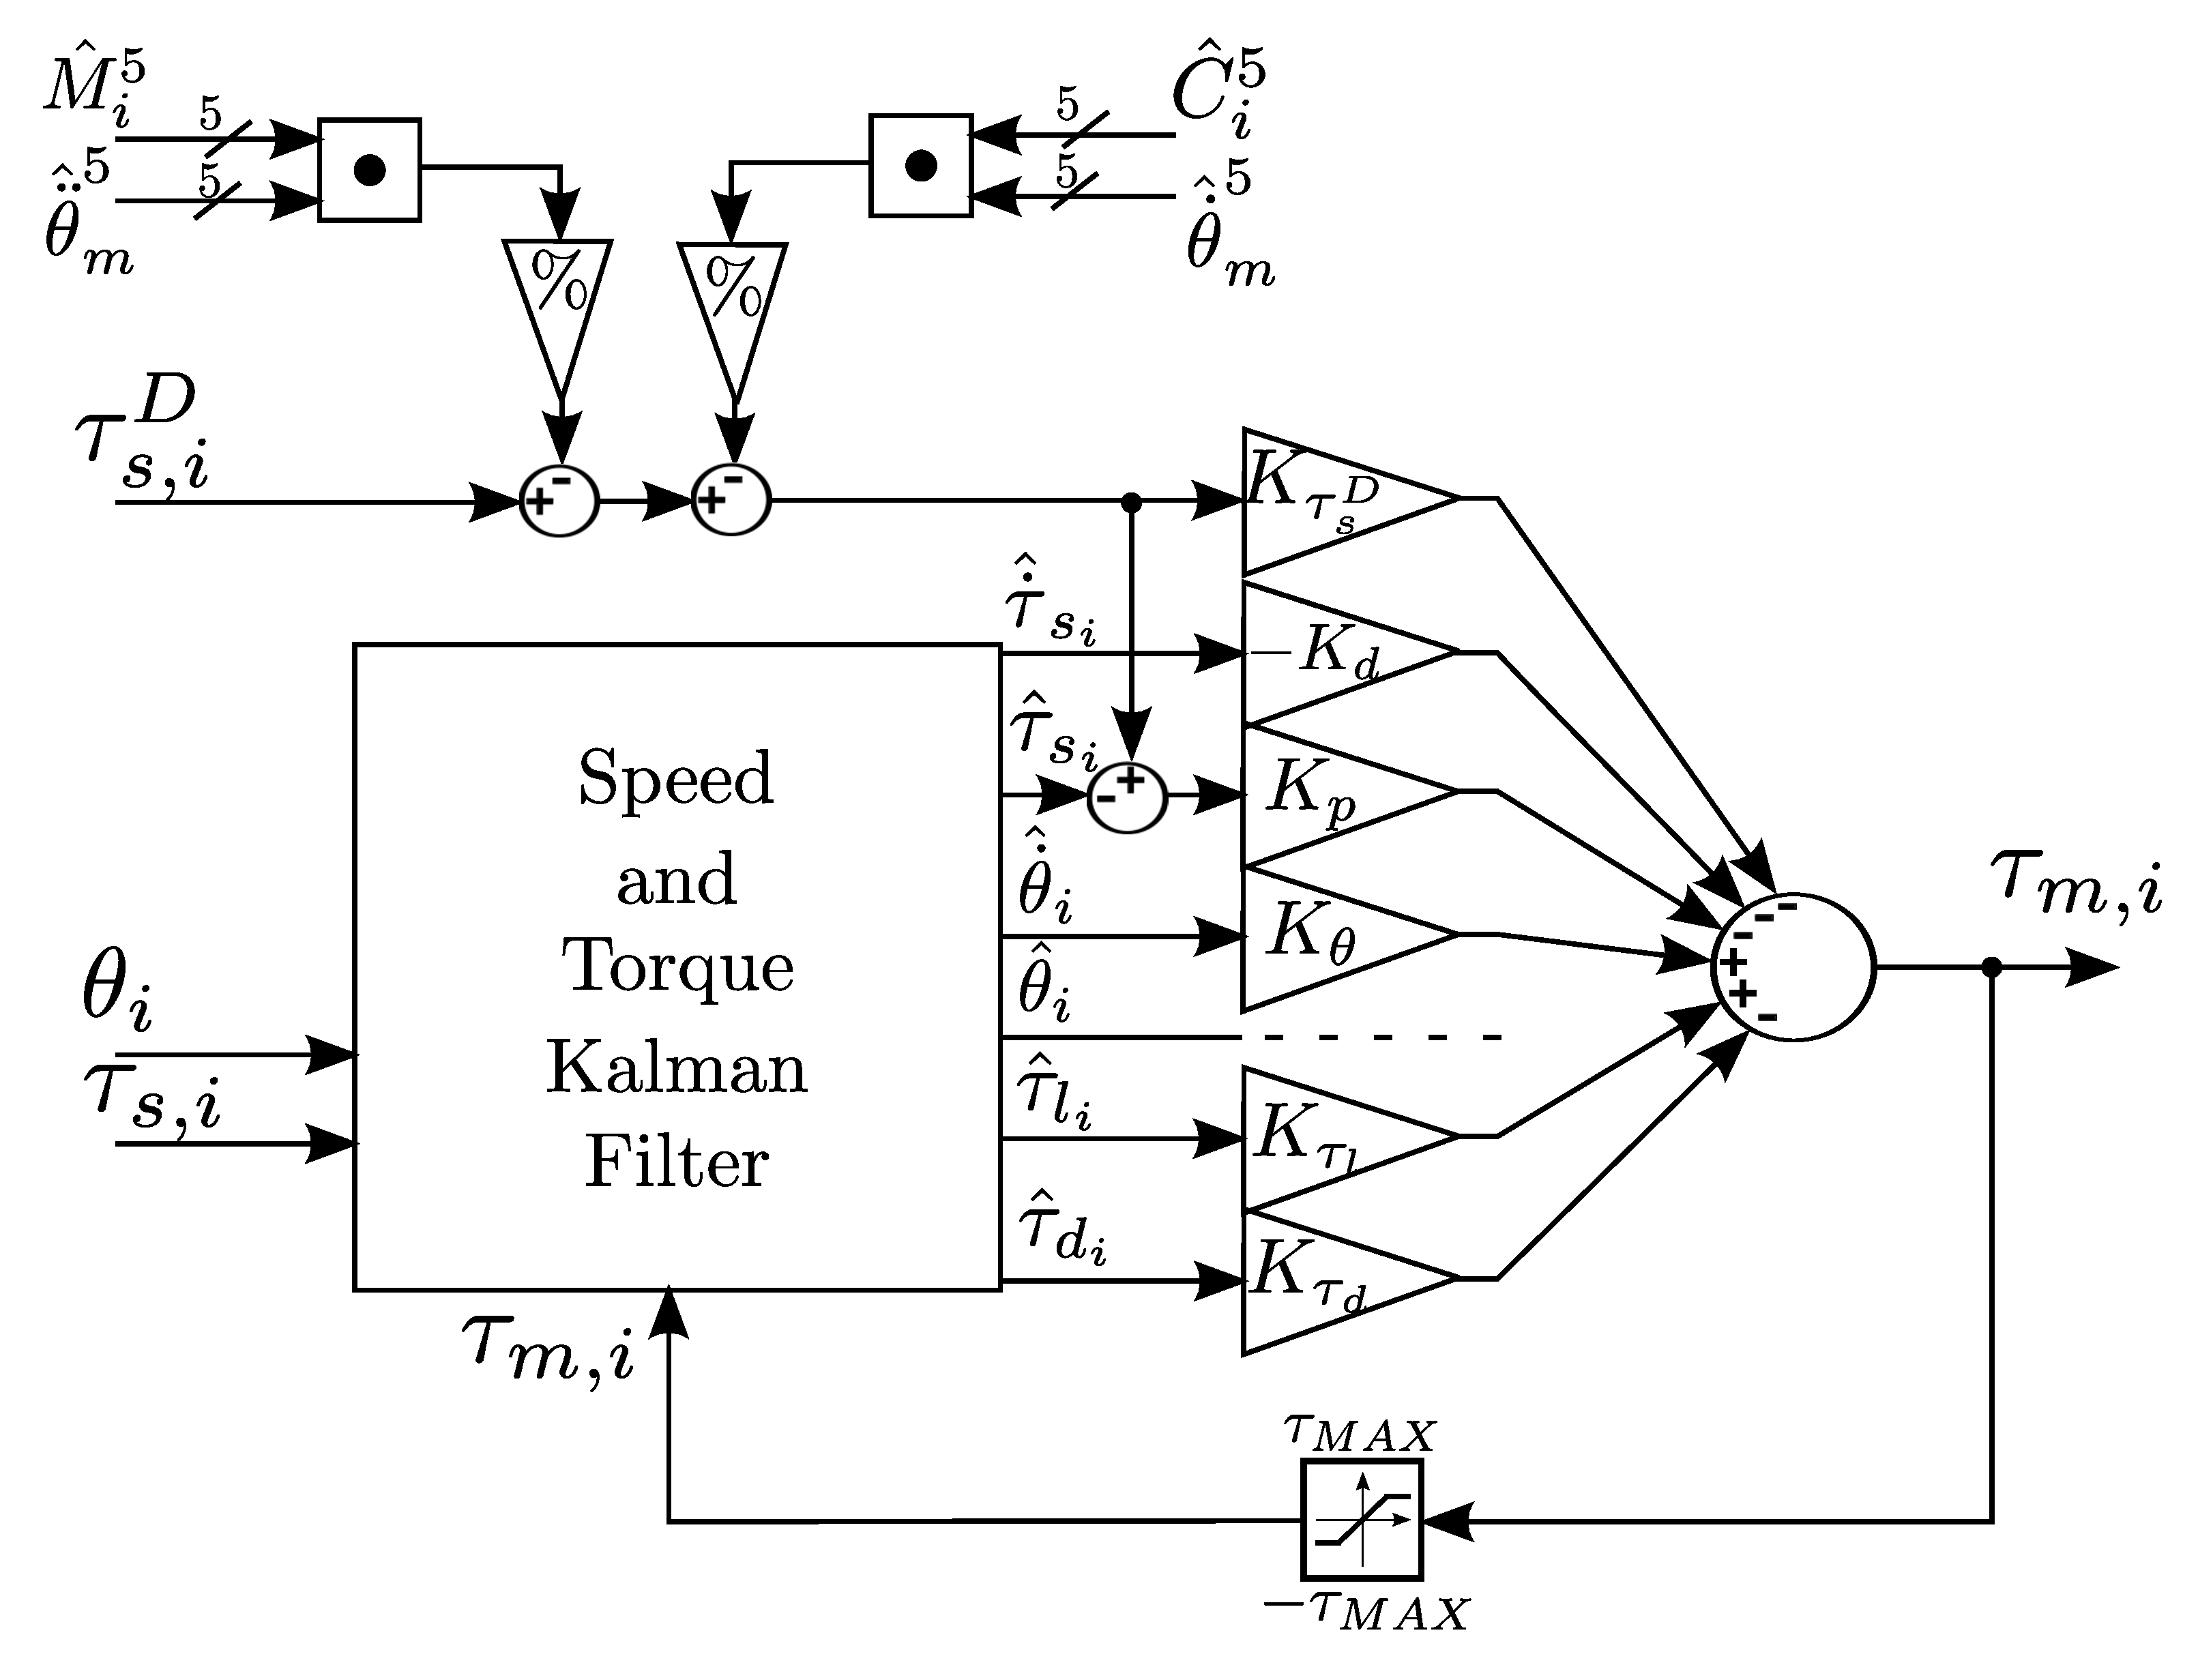
\includegraphics[width=1.0\columnwidth]{FullStateControlFeedback.pdf}
	%DIFDELCMD < 		%%%
	\DIFdelendFL %DIF > 	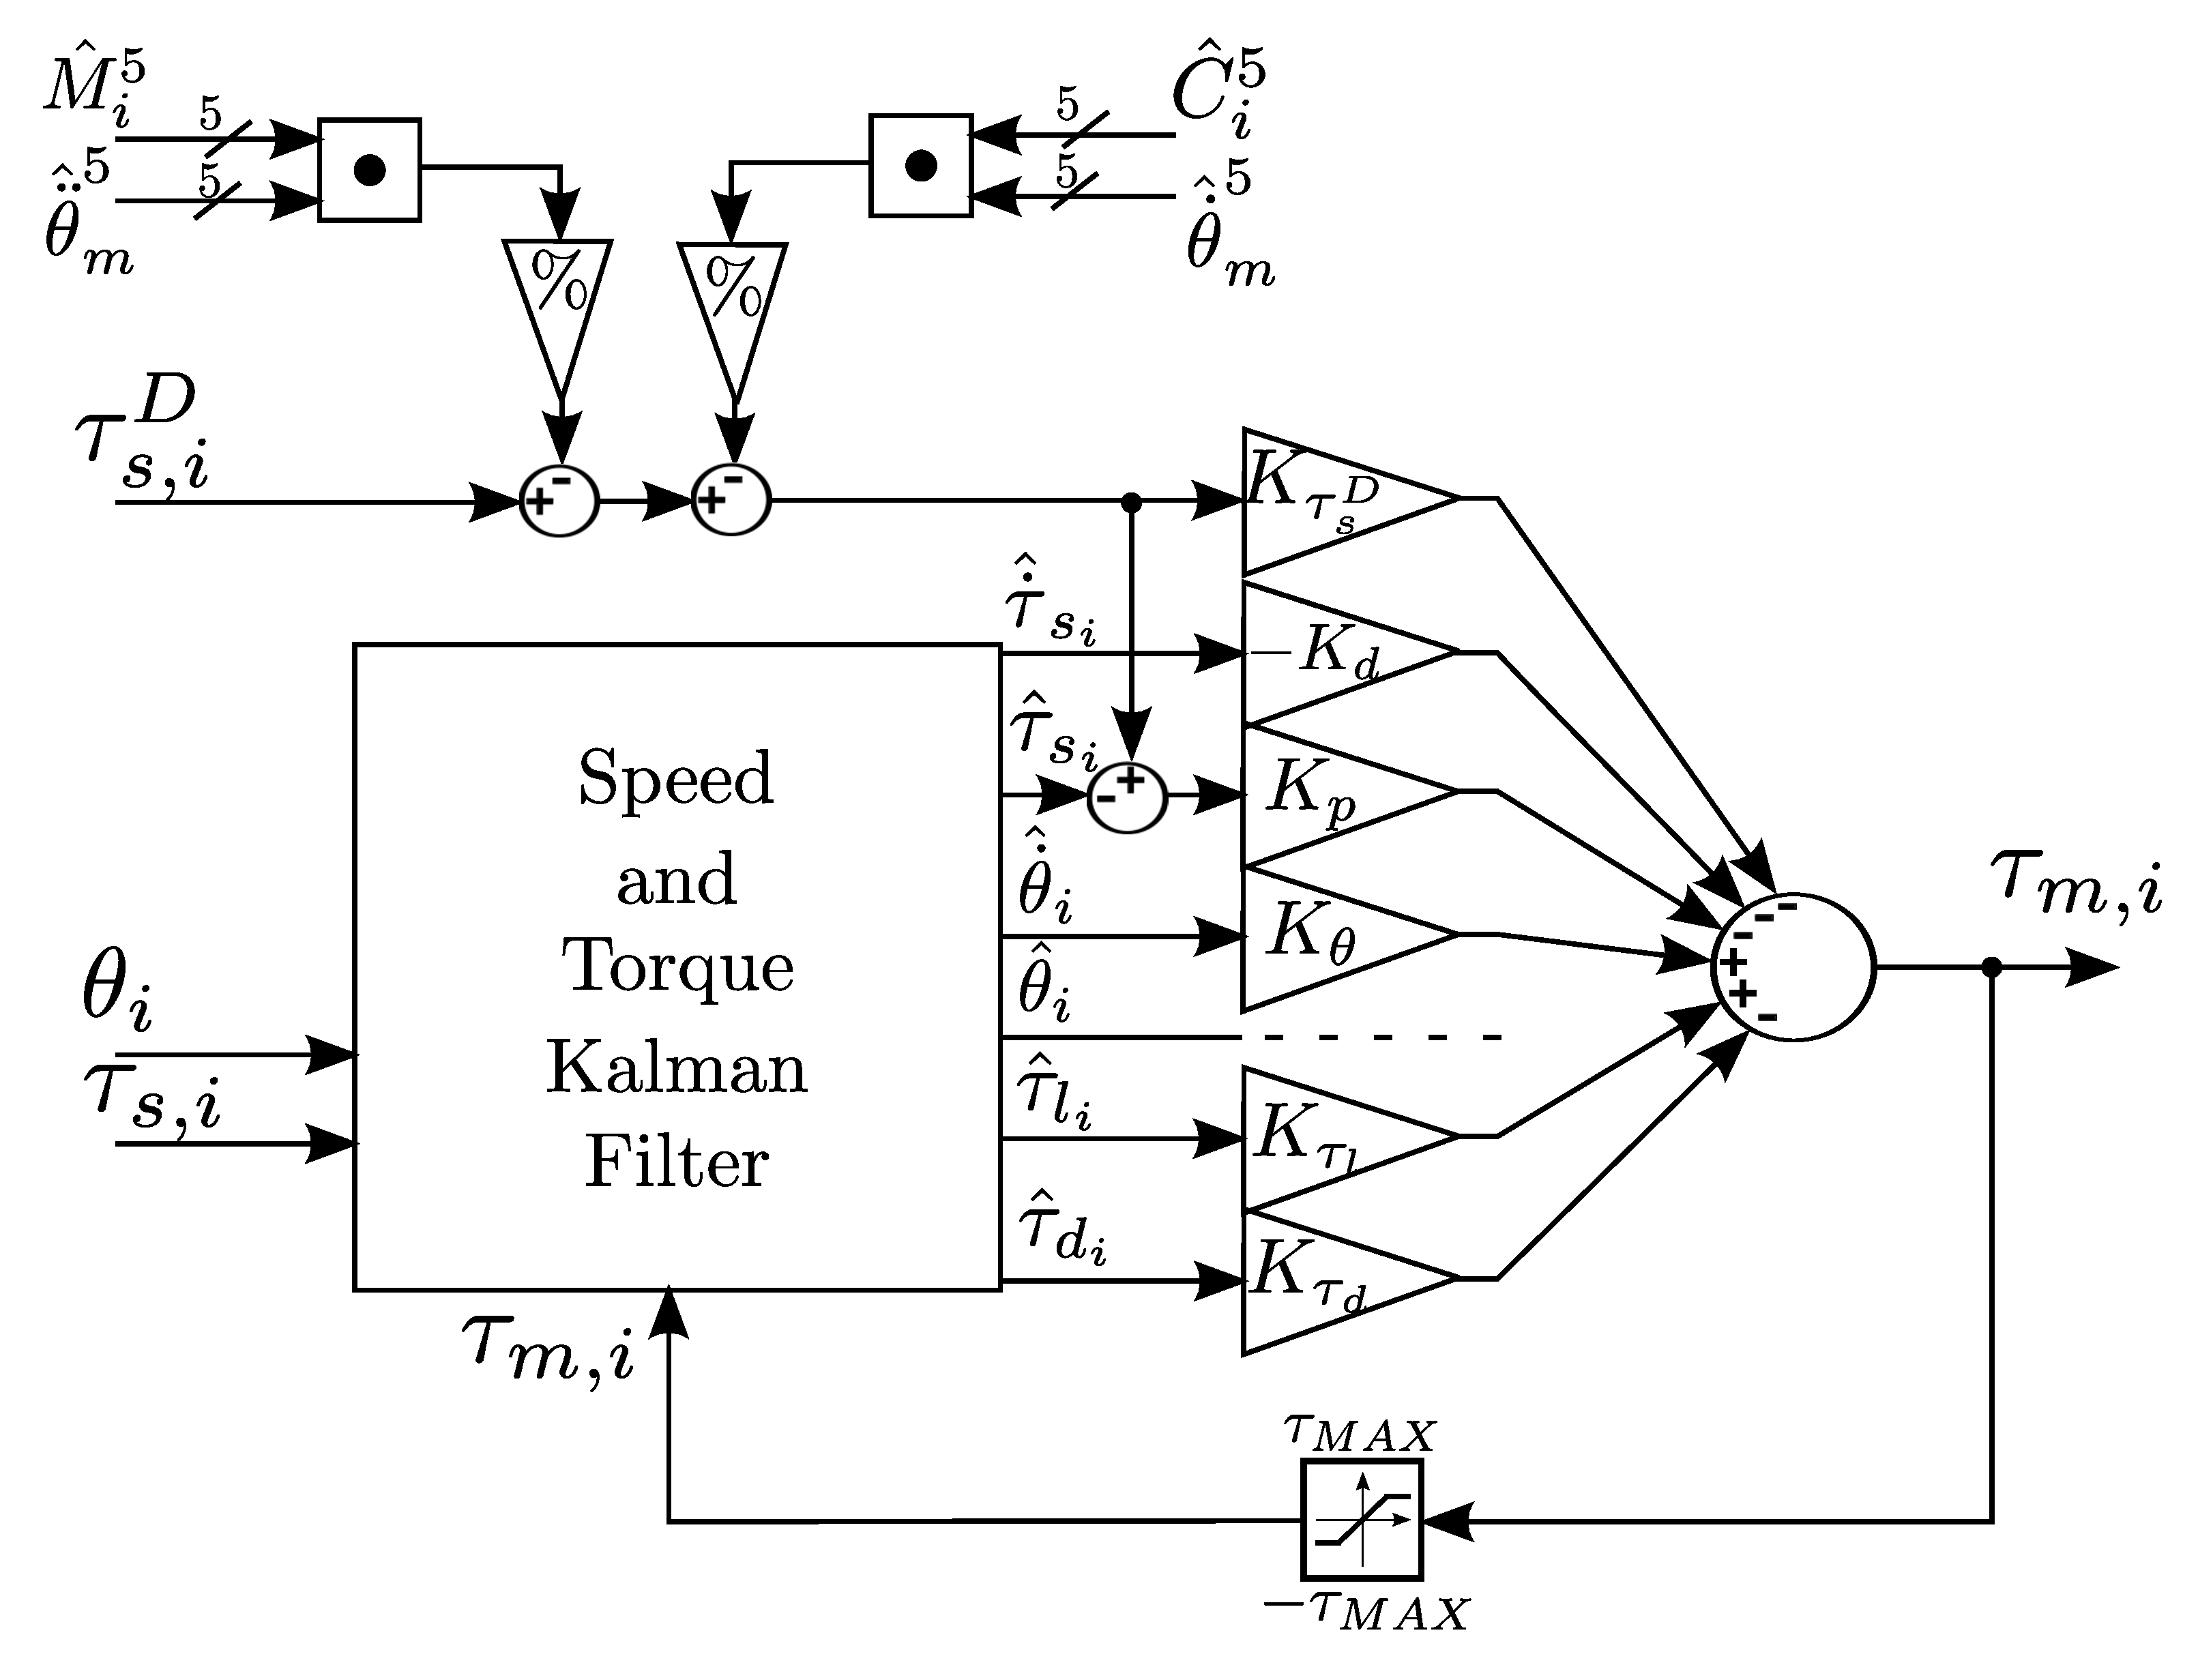
\includegraphics[width=1.0\columnwidth]{FullStateControlFeedback.pdf}
		\DIFaddbeginFL \def\svgwidth{1\columnwidth}
		\begin{footnotesize}
			\input{imgRevised/feedbackController.pdf_tex}
		\end{footnotesize}
		\DIFaddendFL \caption{The schema of the full state control feedback with the dynamic compensation.}
		\DIFdelbeginFL %DIFDELCMD < \label{fig:full state}
	%DIFDELCMD < 	%%%
	\DIFdelendFL \DIFaddbeginFL \label{fig:fullstate}
	\DIFaddendFL \end{figure}
%DIF < \subsubsection{Torque tracking}
%
%\hl{Queste 3 formule} sono già state scritte precedentemente. ATTENZIONE! Scegli dove metterle!
%
%\setlength{\arraycolsep}{0.0em}
%	%DIF < \begin{equation}
%	%DIF < \vects{u_g} = \vects{G}(\vects{D\hat{\theta}_m})
%	%DIF < \label{eq:JTCF1_control_law_a2}
%	%DIF < \end{equation}
%	%DIF < \begin{eqnarray}
%	%DIF < \label{eq:JTCF1_control_law_b2}
%	%DIF < \vects{u_f} = && - \vects{J_m} \vects{K_t}^{-1} \vects{\ddot{\tau}_s^D} + \vects{B_m} \vects{D \dot{\theta}_m} + \vects{J_m} \vects{\overline{M}^{-1}}  \vects{J^T} \vects{\hat{F}_l}  \nonumber \\
%	%DIF < &&{-}\:\vects{\hat{\tau}_d} - {\vects{J}_i^{-1}} \vects{J_m} \vects{\tau_s^D} + \vects{K_p} \vects{e} + \vects{K_d} \vects{\dot{e}}	
%	%DIF < \end{eqnarray}
%	%DIF < \setlength{\arraycolsep}{5pt}
%
%\setlength{\arraycolsep}{0.0em}
%	%DIF < \begin{eqnarray}
%	%DIF < \label{eq:JTCF1_control_law_uf_simple2}
%	%DIF < \vects{u_f} = &&\: \vects{B_m}   \vects{D \dot{\theta}_m} +  \vects{J_m} \vects{\overline{M}^{-1}} \vects{J^T} \vects{\hat{F}_l} - {\vects{J_i^{-1}}} \vects{J_m} \vects{\tau_s^D}  \nonumber \\
%	%DIF < &&{-}\:\vects{\hat{\tau}_d} + \vects{K_p} \vects{e} + \vects{K_d} \vects{\dot{e}}
%	%DIF < \end{eqnarray}
%	%DIF < \setlength{\arraycolsep}{5pt}

%\subsubsection{Impedance control / haptic rendering} \label{subsub:impedanceCJICF2}
%
%For the haptic rendering test, the control law was designed as an impedance control. As internal torque loop was used the law  (\ref{eq:JTCF1_control_law_uf_simple}), while the desired end-effector force $F_{ee}^D$ was chosen as
%%
%\begin{equation}
%	%DIF < \label{eq:desiredVE}
%	%DIF < \left \{
%	%DIF < \begin{aligned}
%	%DIF < & F_{ee}^D = 0, \ \ \ \quad \quad \quad \quad \quad \quad \quad \quad  x < x_d \\
%	%DIF < & F_{ee}^D = \vectm{K_x} (\vects{x - x_d}) - \vectm{D_x}\vects{\dot{x}}, \quad  x \geq x_d  \\
%	%DIF < \end{aligned}
%	%DIF < \right .
%	%DIF < \end{equation}
%%
%%\begin{equation}
%	%DIF < %\tau^D = \vects{K_x} (\vects{x - x_d}) - \vects{D_x J \dot{\theta}} \frac{\vects{x - x_d}}{\left| \vects{x - x_d} \right|}
%	%DIF < %\end{equation}
%%
%obtaining the equivalent torque control law
%%
%\setlength{\arraycolsep}{0.0em}
%	%DIF < \begin{eqnarray}
%	%DIF < \label{eq:JICF1_control_law}
%	%DIF < \vects{u_f} = &&\: \vectm{B_m}  \vectm{D}\vects{\dot{\theta}_m} + \vectm{J_m} \vectm{\overline{M}^{-1}} \vectm{J^T} \vects{F_l} -\vects{\tau_d} \nonumber \\ 
%	%DIF < &&{-}\: {\vectm{J}_i^{-1}} \vectm{J_m J^T}(\vectm{K_x} (\vects{x - x_d}) - \vectm{D_x}\vects{\dot{x}}) \nonumber \\ 
%	%DIF < &&{+}\: \vectm{K_p} \vects{e} + \vectm{K_d} \vects{\dot{e}}
%	%DIF < \end{eqnarray}
%	%DIF < \setlength{\arraycolsep}{5pt}
%%
%where x is coordinate along the normal axis to the surface, $x_d$ is the wall coordinate, $K_x$ and $D_x$ are the desired stiffness and damping respectively of the simulated virtual environment.
%	%DIF < In (\ref{eq:JICF1_control_law}) for the computation of $\vects{J} = \vects{J}(\vects{\bar{\theta}_l})$ and for the gravity compensation term is used $\vects{\bar{\theta}_l} = \vects{D} \vects{\theta_m}$.


%%%%%%%%%%%%%%%%%%%%%%%%%%%%%%%%%%%%%%%%%%%%%%%%%%%%%%%%%%%%%%%%%%%%%%%%%%%%%%%%%%%%%%%%%%%%%%%%%%%%%%%%%%%%%%%%%%%%
%%%%%%%%%%%%%%%%%%%%%%%%%%%%%%%%%%%%%%%%%%%%%%%%%%%%%%%%%%%%%%%%%%%%%%%%%%%%%%%%%%%%%%%%%%%%%%%%%%%%%%%%%%%%%%%%%%%%
\subsection{A basic state feedback controller (JTFC2)} \label{subsec:JTFC2}

The basic state feedback controller is derived assuming the following full model dynamics\DIFdelbegin \DIFdel{(extended the one }\DIFdelend \DIFaddbegin \DIFadd{, extending the model }\DIFaddend introduced for a single joint by Hashimoto \cite{hashimoto1998experimental} \DIFdelbegin \DIFdel{), that }\DIFdelend \DIFaddbegin \DIFadd{where feedforward compensation using desired
	torque is presented for  torque control using harmonic drive built-in torque sensor. The JTFC2 model  }\DIFaddend differs from (\ref{eqn:dinamicaLinkMultiGiunto})  \DIFdelbegin \DIFdel{for the absence of external forces:
}\DIFdelend \DIFaddbegin \DIFadd{since has no damping contribution of the elastic transmission and external forces.
}\DIFaddend 

%\setlength{\arraycolsep}{0.0em}
%DIF < \begin{eqnarray}
%DIF < \label{eq:JICF1_control_law}
%DIF < \vects{u_f} = &&\: \vects{B_m}  \vects{D \dot{\theta}_m} + \vects{J_m} \vects{\overline{M}^{-1}} \vects{J^T} \vects{F_l} -\vects{\tau_d} \nonumber \\ 
%DIF < &&{-}\: {\vects{J}_i^{-1}} \vects{J_m J^T}(\vects{K_x} (\vects{x - x_d}) - \vects{D_x J \dot{\theta}} \frac{\vects{x - x_d}}{\left| \vects{x - x_d} \right|}) \nonumber \\ 
%DIF < &&{+}\: \vects{K_p} \vects{e} + \vects{K_d} \vects{\dot{e}}
%DIF < \end{eqnarray}
%DIF < \setlength{\arraycolsep}{5pt}
 %%%%%%%%%%%%%%%%%%%%%%%%%%%%%%%%%%%%%%%%%%%%%%%%%%%%%%%%%%%%%%%%%%%%%%%%%%%%%%%%%%%%%%%%%%%%%%%%%%%%%%%%%%%%%%%%%%%%
%%%%%%%%%%%%%%%%%%%%%%%%%%%%%%%%%%%%%%%%%%%%%%%%%%%%%%%%%%%%%%%%%%%%%%%%%%%%%%%%%%%%%%%%%%%%%%%%%%%%%%%%%%%%%%%%%%%%
%%%xxxxxxxxxxxxxxx%%%%%%%%%%%%%%%%


\hl{SUBMITTED VERSION}

\hl{REVISED VERSION}


\DIFdelbegin \DIFdel{Assuming the above full model dynamics, the input control $\vects{u}$ is designed as in (\ref{generic_control_law1}), where for $\vects{u}_g$ is used (\ref{eq:JTCF1_control_law_a}).
}\DIFdelend %DIF > Assuming the above full model dynamics, the input control $\vects{u}$ is designed as in (\ref{generic_control_law1}), where for $\vects{u}_g$ is used (\ref{eq:JTCF1_control_law_a}).
\%DIFaddbegin 



\DIFaddend %\begin{equation}
%DIF < \label{generic_control_law2}
%DIF < \vects{u}  =  \vects{u_f} + \vects{u_g}
%DIF < \end{equation}
%DIF < 
%DIF < For $\vects{u}_g$ is used (\ref{eq:JTCF1_control_law_a}). %\hl{oppure una stima del tipo $G(K^{-1}_t \tau_s - D \theta_m)$}. \\
%DIF > For $\vects{u}_g$ is used (\ref{eq:JTCF1_control_law_a}). %\hl{oppure una stima del tipo $G(K^{-1}_t \uptau_s - D \uptheta_m)$}. \\
%
%The basic control law used in \cite{hashimoto1998experimental} can be generalized in case of multi-joint robot and, according to the  proposed notation, it is
%
%\setlength{\arraycolsep}{0.0em}
%DIF < \begin{eqnarray}
%DIF < \label{JTFC2_uf_control_law_noSimplified}
%DIF < \vects{u_f} = &&\: -\vectm{J_m} \vectm{{K^{-1}_t}} ( - \vects{{\ddot{\tau}^D}_s} - \vectm{J^{-1}_i} \vectm{J_m} \vects{{\tau^D}_s} - \vectm{K_d}(\vects{\dot{\tau}_s} - \vects{{\dot{\tau}^D}_s}) \nonumber \\ 
%DIF < &&\: -\vectm{K_p}(\vects{\tau_s} - \vects{\tau^D_s})) 
%DIF > \vects{u_f} = &&\: -\vectm{J_m} \vectm{{K^{-1}_t}} ( - \vects{{\ddot{\uptau}^D}_s} - \vectm{J^{-1}_i} \vectm{J_m} \vects{{\uptau^D}_s} - \vectm{K_d}(\vects{\dot{\uptau}_s} - \vects{{\dot{\uptau}^D}_s}) \nonumber \\ 
%DIF > &&\: -\vectm{K_p}(\vects{\uptau_s} - \vects{\uptau^D_s})) 
%\end{eqnarray}
%DIF < \setlength{\arraycolsep}{5pt}

The basic control law used in \cite{hashimoto1998experimental} can be generalized in case of multi-joint robot. Thus \DIFdelbegin \DIFdel{, according to the proposed notation , if one assumes  $\vects{e}=\vects{\tau_s}-\vects{\tau_s^D}$ as the error on sensor torque, given the desired sensor torque  $\vects{\tau_s^D}$, ans one assume moreover that $\vects{\dot{\tau}^D}=\vects{0}$ and $\vects{\ddot{\tau}^D}=\vects{0}$, so that 
	$\vects{\dot{e}}=\vects{\dot{\tau}_s}$ }\DIFdelend \DIFaddbegin \DIFadd{using the same notation }\DIFaddend and \DIFdelbegin \DIFdel{$\vects{\ddot{e}}=\vects{\ddot{\tau}_s}$, }\DIFdelend \DIFaddbegin \DIFadd{conditions of }\eqref{eq:conditions}\DIFadd{, }\DIFaddend the control law \DIFaddbegin \DIFadd{$\vects{u}_f$  }\DIFaddend can be written as \DIFaddbegin \DIFadd{a function of desired torque, where for $\vects{u}_g$ is used (\ref{eq:JTCF1_control_law_uf_simple}):
	%DIF > according to the  proposed notation, if one assumes  $\vect{e}=\vects{\uptau_s}-\vects{\uptau_s^D}$ as the error on sensor torque, given the desired sensor torque  $\vects{\uptau_s^D}$, ans one assume moreover
	%DIF >  that $\vects{\dot{\uptau}^D}=\vect{0}$ and  $\vects{\ddot{\uptau}^D}=\vect{0}$, so that 
	%DIF > $\vect{\dot{e}}=\vects{\dot{\uptau}_s}$ and  $\vect{\ddot{e}}=\vects{\ddot{\uptau}_s}$, 
}\DIFaddend 





\setlength{\arraycolsep}{0.0em}
\begin{equation}
\label{JTFC2_control_law_final}
\DIFdelbegin %DIFDELCMD < \vects{u_f} %%%
\DIFdelend \DIFaddbegin \vect{u_f} \DIFaddend = - \DIFdelbegin %DIFDELCMD < \vectm{J^{-1}_i} \vectm{J_m} \vects{\tau^D_s} %%%
\DIFdel{+ }%DIFDELCMD < \vectm{J_m} \vectm{K^{-1}_t} \vectm{K_d} \vects{\dot{e}} %%%
\DIFdel{+ }%DIFDELCMD < \vectm{J_m} \vectm{K^{-1}_t} \vectm{K_p} \vects{e} 
%DIFDELCMD < %%%
\  DIFdelend \DIFaddbegin \underbrace{\colorboxed{green}{\vectm{I^{-1}_i} \vectm{I_m} \vects{\uptau^D_s}}}\DIFadd{_{\text{desired torque}}
	- }\underbrace{\colorboxed{red}{\vectm{I_m} \vectm{K^{-1}_t} (\vects{\ddot{\uptau}_s^D}- \vectm{K_d} \vect{\dot{e}} -  \vectm{K_p} \vect{e}  )}}\DIFadd{_{\text{state feedback}}
}\DIFaddend \end{equation}
\setlength{\arraycolsep}{5pt}



The modified dynamics with the control law  (\ref{JTFC2_control_law_final}), leads to the following error dynamics \DIFdelbegin \DIFdel{equations}\DIFdelend \DIFaddbegin \DIFadd{equation}\DIFaddend :

\setlength{\arraycolsep}{0.0em}
\DIFdelbegin \begin{eqnarray*}\DIFdel{
		\label{JTFC2_error_equation1}
		\vects{\ddot{\theta}_m} }&\DIFdel{= \vectm{D^{-1}} \vects{\ddot{\theta}_l} - \vectm{D^{-1}} \vectm{K_t^{-1}} \vects{\ddot{e}}
	}\\
	\DIFdel{\label{JTFC2_error_equation2}
		\vectm{J^T} \vects{F_l} - \vectm{K_t} \vectm{J^{-1}_m} \vects{\tau_d}}& \DIFdel{= \vects{\ddot{e}} + \vectm{K_d} \vects{\dot{e}} + (\vectm{K_p} + \vectm{J^{-1}_i} \vectm{K_t}) \vects{e}
	}\end{eqnarray*}
	%DIFAUXCMD
	\DIFdelend \DIFaddbegin \begin{IEEEeqnarraybox}[][c]{l}
		%DIF > \label{JTFC2_error_equation1}
		%DIF > \vects{\ddot{\uptheta}_m} &= \vectm{D^{-1}} \vects{\ddot{\uptheta}} - \vectm{D^{-1}} \vectm{K_t^{-1}} \vects{\ddot{e}}
		%DIF > \\
		\label{JTFC2_error_equation2}
		\vectm{K_t}   \overline{\vectm{M}}\DIFadd{^{-1}   }\vectm{J^T} \vect{F_l} \DIFadd{+ }\vectm{B_m D}\vects{\dot{\uptheta}_m}\DIFadd{- }\vectm{K_t} \vectm{I^{-1}_m} \vects{\uptau_d} \\\DIFadd{= }\vect{\ddot{e}} \DIFadd{+ (}\vectm{K_d} \DIFadd{+ }\vectm{I^{-1}_i} \vectm{C_t}\DIFadd{) }\vect{\dot{e}} \DIFadd{+ (}\vectm{K_p} \DIFadd{+ }\vectm{I^{-1}_i} \vectm{K_t}\DIFadd{) }\vect{e}
	\end{IEEEeqnarraybox}
	\DIFaddend \setlength{\arraycolsep}{5pt}
	
	%DIF > HOW IT SHOULD BE THE NEW EQUATION
	%DIF > 
	%DIF > \setlength{\arraycolsep}{0.0em}
	%DIF > 	\begin{IEEEeqnarraybox}[][c]{l}
	%DIF > %\label{JTFC2_error_equation1}
	%DIF > %\vects{\ddot{\uptheta}_m} &= \vectm{D^{-1}} \vects{\ddot{\uptheta}} - \vectm{D^{-1}} \vectm{K_t^{-1}} \vects{\ddot{e}}
	%DIF > %\\
	%DIF > \label{JTFC2_error_equation2}
	%DIF > \vectm{K_t}   \overline{\vectm{M}}^{-1}   \vectm{J^T} \vect{F_l} + \vectm{B_m D}\vects{\dot{\uptheta}_m}- \vectm{K_t} \vectm{I^{-1}_m} \vects{\uptau_d} \\= \vects{\ddot{e}} + (\vectm{K_d} + \vectm{I^{-1}_i} \vectm{C_t}) \vects{\dot{e}} + (\vectm{K_p} + \vectm{I^{-1}_i} \vectm{K_t}) \vects{e}
	%DIF > \end{IEEEeqnarraybox}
	%DIF > \setlength{\arraycolsep}{5pt}
	\DIFaddbegin 
	
	
	
	
	
	
	
	%DIF > ****************************
	%DIF > EQUATION VERIFICATION
	%DIF > 
	%DIF > %\footnotesize
	%DIF > \begin{equation}
	%DIF > \boxed{
	%DIF > 	\left
	%DIF > 	\{
	%DIF > 	\begin{IEEEeqnarraybox}[][c]{l}
	%DIF > 	\vects{\ddot{\uptau}_s}  + \vectm{C_t I_i}^{-1} \vects{\dot{\uptau}_s} + \vectm{K_t I_i}^{-1} \vects{\tau_s}= \vectm{K_t I_{m}}^{-1} (\vectm{I_{m}} \overline{\vectm{M}}^{-1}  \vectm{J}^T \vects{F_l}  +  \vectm{B_m D}\vects{\dot{\uptheta}_m} \\
	%DIF > 	{+}\:  \vectm{B_m D}\vects{\dot{\uptheta}_m}-\vects{\uptau_d} - \vect{u})
	%DIF > 	\end{IEEEeqnarraybox}
	%DIF > 	\right .
	%DIF > }
	%DIF > \end{equation}
	%DIF > \normalsize
	%DIF > %\label{eq:dynamics_eq1}
	%DIF > %\label{eq:dynamics_eq2}
	%DIF > \setlength{\arraycolsep}{0.0em}
	%DIF > 
	%DIF > 
	%DIF > 
	%DIF > 
	%DIF > %\footnotesize
	%DIF > \begin{equation}
	%DIF > \boxed{
	%DIF > 	\left
	%DIF > 	\{
	%DIF > 	\begin{IEEEeqnarraybox}[][c]{l}
	%DIF > 	\vects{\ddot{\uptau}_s}  + \vectm{C_t I_i}^{-1} \vects{\dot{\uptau}_s} + \vectm{K_t I_i}^{-1} \vects{\tau_s}= \vectm{K_t I_{m}}^{-1} (\vectm{I_{m}} \overline{\vectm{M}}^{-1}  \vectm{J}^T \vects{F_l}  +  \\
	%DIF > 	{+}\:  \vectm{B_m D}\vects{\dot{\uptheta}_m}-\vects{\uptau_d}  \\
	%DIF > +	\underbrace{\colorboxed{green}{\vectm{I^{-1}_i} \vectm{I_m} \vects{\uptau^D_s}}}_{\text{desired torque}}
	%DIF > 	+ \underbrace{\colorboxed{red}{\vectm{I_m} \vectm{K^{-1}_t} (\vects{\ddot{\uptau}_s^D}- \vectm{K_d} \vect{\dot{e}} -  \vectm{K_p} \vect{e}  )}}_{\text{state feedback}})
	%DIF > 	\end{IEEEeqnarraybox}
	%DIF > 	\right .
	%DIF > }
	%DIF > \end{equation}
	%DIF > \normalsize
	%DIF > %\label{eq:dynamics_eq1}
	%DIF > %\label{eq:dynamics_eq2}
	%DIF > \setlength{\arraycolsep}{0.0em}
	%DIF > 
	%DIF > 
	%DIF > 
	%DIF > 
	%DIF > 
	%DIF > %\footnotesize
	%DIF > \begin{equation}
	%DIF > \boxed{
	%DIF > 	\left
	%DIF > 	\{
	%DIF > 	\begin{IEEEeqnarraybox}[][c]{l}
	%DIF > 	\vects{\ddot{\uptau}_s}  + \vectm{C_t I_i}^{-1} \vects{\dot{\uptau}_s} + \vectm{K_t I_i}^{-1} \vects{\tau_s}= \vectm{K_t I_{m}}^{-1} (\vectm{I_{m}} \overline{\vectm{M}}^{-1}  \vectm{J}^T \vects{F_l}  +  \\
	%DIF > 	{+}\:  \vectm{B_m D}\vects{\dot{\uptheta}_m}-\vects{\uptau_d}  \\
	%DIF > 	+	\underbrace{\colorboxed{green}{\vectm{I^{-1}_i} \vectm{I_m} \vects{\uptau^D_s}}}_{\text{desired torque}})
	%DIF > 	+ \underbrace{\colorboxed{red}{ (\vects{\ddot{\uptau}_s^D}- \vectm{K_d} \vect{\dot{e}} -  \vectm{K_p} \vect{e}  )}}_{\text{state feedback}})
	%DIF > 	\end{IEEEeqnarraybox}
	%DIF > 	\right .
	%DIF > }
	%DIF > \end{equation}
	%DIF > \normalsize
	%DIF > %\label{eq:dynamics_eq1}
	%DIF > %\label{eq:dynamics_eq2}
	%DIF > \setlength{\arraycolsep}{0.0em}
	%DIF > 
	%DIF > **********************************
	
	\DIFaddend %\subsubsection{Torque tracking}
	%
	%\setlength{\arraycolsep}{0.0em}
	%\begin{eqnarray}
	%DIF < \label{JTFC2_control_law_noSimplified}
	%DIF < \vects{u_f} = &&{-}\: \vects{J_m} \vects{K^{-1}_t} ( -\vects{\ddot{\tau}^D_s} - \vects{J^{-1}_i} \vects{J_m} \vects{\tau^D_s} - \vects{K_d} (\vects{\dot{\tau}_s} - \vects{\dot{\tau}^D_s})  \nonumber \\
	%DIF < &&{-}\: \vects{K_p}(\vects{\tau_s} - \vects{\tau^D_s})) 
	%DIF < DIF < \end{eqnarray}
	%DIF < \setlength{\arraycolsep}{5pt}
	%
	%DIF < If one assume  $\vects{e}=\vects{\tau_s}-\vects{\tau_s^D}$ as the error on sensor torque, given the desired sensor torque  $\vects{\tau_s^D}$, ans one assume moreover that $\vects{\dot{\tau}^D}=\vects{0}$ and  $\vects{\ddot{\tau}^D}=\vects{0}$,
	%DIF < DIF < so that 
	%DIF < $\vects{\dot{e}}=\vects{\dot{\tau}_s}$ and  $\vects{\ddot{e}}=\vects{\ddot{\tau}_s}$, the (\ref{JTFC2_control_law_noSimplified}) can be rewritten as
	%
	%DIF < \begin{equation}
	%DIF < \label{JTFC2_control_law}
	%DIF < DIF < \vects{u_f} = - \vects{J^{-1}_i} \vects{J_m} \vects{\tau^D_s} + \vects{J_m} \vects{K^{-1}_t} \vects{K_d} \vects{\dot{e}} + \vects{J_m} \vects{K^{-1}_t} \vects{K_p} \vects{e}
	%\end{equation}
	
	%\subsubsection{Impedance control / haptic rendering}
	%
	%DIF < The impedance control law for the JTFC2 uses the same desired end-effector force as in (\ref{eq:desiredVE}) that leads to the equivalent torque control law
	%%
	%DIF < \setlength{\arraycolsep}{0.0em}
	%DIF < \begin{eqnarray}
	%DIF < \label{eq:JICF2_control_law}
	%DIF < \vects{u_f} = &&{-}\: \vectm{J^{-1}_i} \vectm{J_m J^T}(\vectm{K_x} (\vects{x - x_d}) - \vectm{D_x}\vects{\dot{x}}) \nonumber \\
	%DIF < &&{+}\: \vectm{J_m}  \vectm{K^{-1}_t} \vectm{K_d} \vects{\dot{e}} + \vectm{J_m} \vectm{K^{-1}_t} \vectm{K_p} \vects{e} 
	%DIF < DIF < \end{eqnarray}
	%DIF < \setlength{\arraycolsep}{5pt}
	%%%           < 
	\DIFdelend \DIFdelend %whit the same terms' meaning.
	%%%%%%%%%%%%%%%%%%%%%%%%%%%%%%%%%%%%%%%%%%%%%%%%%%%%%%%%%%%%%%%%%%%%%%%%%%%%%%%%%%%%%%%%%%%%%%%%%%%%%%%%%%%%%%%%%%%%
	%%%%%%%%%%%%%%%%%%%%%%%%%%%%%%%%%%%%%%%%%%%%%%%%%%%%%%%%%%%%%%%%%%%%%%%%%%%%%%%%%%%%%%%%%%%%%%%%%%%%%%%%%%%%%%%%%%%%
	\subsection{A passivity-based feedback controller (JTFC3)} \label{subsec:JTFC3}
	
	The passivity-based state feedback is derived assuming the following full model dynamics (introduced by Ott in \cite{kugi2008passivity}), that differs from  (\ref{eqn:dinamicaLinkMultiGiunto}) for the absence of the motor's viscous friction term \DIFdelbegin \DIFdel{:
	}\DIFdelend \DIFaddbegin \DIFadd{$\vectm{B_m } \vectm{D} \vects{\dot{\uptheta}_m} $. 
	%DIF > and modeling of disturbance forces $\vects{\uptau_d} $:
}\DIFaddend 


\DIFdelbegin %DIFDELCMD < \footnotesize
%DIFDELCMD < %%%
\begin{displaymath}\DIFdel{
	\left \{
	\begin{IEEEeqnarraybox}[][c]{l}
	\label{dynamic_model_modifiedKugi_1}
	\vectm{J_m}  \vectm{D} \vects{\ddot{\theta}_m} + \vectm{C_t}(\vectm{D}\vects{\dot{\theta}_m} - \vects{\dot{\theta}_j}) + \vectm{K_t}(\vectm{D}\vects{\theta_m} - \vects{\theta_j}) = \vects{\tau_m}  }\\
  \DIFdel{\vectm{M}(\vects{\theta_j}) \vects{\ddot{\theta}_j} }{\DIFdel{+}}\DIFdel{\: \vectm{C}(\vects{\dot{\theta}_j},\vects{\theta_j}) \vects{\dot{\theta}_j} + \vectm{C_t}(\vects{\dot{\theta}_j} - \vectm{D}\vects{\dot{\theta}_m})  }{\DIFdel{+}}\DIFdel{\: \vects{G}(\vects{\theta_j})+}\\
\DIFdel{+ \vectm{K}(\vects{\theta_j} - \vectm{D}\vects{\theta_m}) = \vectm{J^T} \vects{F_h} 
	\end{IEEEeqnarraybox}
	\right . %DIF < \label{eqn:dinamicaMotoreMultiGiunto}
}\end{displaymath}


%DIFAUXCMD
%DIFDELCMD < \normalsize
%DIFDELCMD < 

%DIFDELCMD < \setlength{\arraycolsep}{0.0em}
%DIFDELCMD < %%%
\DIFdelend %DIF > 
%DIF > %\footnotesize
%\begin{equation}
%DIF > \left \{
%DIF > \begin{IEEEeqnarraybox}[][c]{l}
%\label{dynamic_model_modifiedKugi_1}
%DIF < \vectm{J_m}  \vectm{D} \vects{\ddot{\theta}_m} + \vectm{C_t}(\vectm{D}\vects{\dot{\theta}_m} - \vects{\dot{\theta}_j}) + \vectm{K_t}(\vectm{D}\vects{\theta_m} - \vects{\theta_j}) = \vects{\tau_m} 
%DIF > \vectm{I_m}  \vectm{D} \vects{\ddot{\uptheta}_m} + \vectm{C_t}(\vectm{D}\vects{\dot{\uptheta}_m} - \vects{\dot{\uptheta}}) + \vectm{K_t}(\vectm{D}\vects{\uptheta_m} - \vects{\uptheta_j}) = \vects{\uptau_m}  \\
%DIF > \vectm{M}(\vects{\uptheta}) \vects{\ddot{\uptheta}} {+}\: \vectm{C}(\vects{\dot{\uptheta}},\vects{\uptheta}) \vects{\dot{\uptheta}} + \vectm{C_t}(\vects{\dot{\uptheta}} - \vectm{D}\vects{\dot{\uptheta}_m})   +\vectm{K_t}(\vects{\uptheta} - \vectm{D}\vects{\uptheta_m}) +\\
%DIF >  + \vects{G}(\vects{\uptheta})  = \vectm{J^T} \vects{F_h} 
%DIF > \end{IEEEeqnarraybox}
%DIF > \right . %\label{eqn:dinamicaMotoreMultiGiunto}
%\end{equation}
%DIF > \normalsize
%DIF > 
%DIF > 
%DIF > \setlength{\arraycolsep}{0.0em}
%DIF > \begin{equation}
%DIF > \label{dynamic_model_modifiedKugi_1}
%DIF > \vectm{J_m}  \vectm{D} \vects{\ddot{\uptheta}_m} + \vectm{C_t}(\vectm{D}\vects{\dot{\uptheta}_m} - \vects{\dot{\uptheta}_j}) + \vectm{K_t}(\vectm{D}\vects{\uptheta_m} - \vects{\uptheta_j}) = \vects{\uptau_m} 
%DIF > \end{equation}
%\begin{eqnarray}
%\label{dynamic_model_modifiedKugi_2}
%DIF < \vectm{M}(\vects{\theta_j}) \vects{\ddot{\theta}_j} &&{+}\: \vectm{C}(\vects{\dot{\theta}_j},\vects{\theta_j}) \vects{\dot{\theta}_j} + \vectm{C_t}(\vects{\dot{\theta}_j} - \vectm{D}\vects{\dot{\theta}_m}) \nonumber \\
%DIF < &&{+}\: \vects{G}(\vects{\theta_j}) + \vectm{K}(\vects{\theta_j} - %\vectm{D}\vects{\theta_m}) = \vectm{J^T} \vects{F_h} 
%DIF > \vectm{M}(\vects{\uptheta_j}) \vects{\ddot{\uptheta}_j} &&{+}\: \vectm{C}(\vects{\dot{\uptheta}_j},\vects{\uptheta_j}) \vects{\dot{\uptheta}_j} + \vectm{C_t}(\vects{\dot{\uptheta}_j} - \vectm{D}\vects{\dot{\uptheta}_m}) \nonumber \\
%DIF > &&{+}\: \vects{G}(\vects{\uptheta_j}) + \vectm{K}(\vects{\uptheta_j} - %\vectm{D}\vects{\uptheta_m}) = \vectm{J^T} \vects{F_h} 
%\end{eqnarray}
\DIFdelbegin \begin{displaymath}\DIFdel{
	\label{dynamic_model_modifiedKugi_3}
	\vects{\tau_s} = - \vectm{K_t} (\vectm{D} \vects{\theta_m} - \vects{\theta_j})
}\end{displaymath}
%DIFAUXCMD
%DIFDELCMD < \setlength{\arraycolsep}{5pt}
%DIFDELCMD < %%%
\DIFdelend %DIF > \begin{equation}
%DIF > \label{dynamic_model_modifiedKugi_3}
%DIF > \vects{\uptau_s} = - \vectm{K_t} (\vectm{D} \vects{\uptheta} - \vects{\uptheta_j})
%DIF > \end{equation}
%DIF > \setlength{\arraycolsep}{5pt}
%
%In \cite{kugi2008passivity} the control law is
%
%\begin{equation}
%\label{generic_control_law3}
%\vects{u} =  \vects{u_f} + \vects{u_g}
%\end{equation}

%DIF > 
%DIF > **************************************************
%DIF > %%%EQUIVALENT MODEL
%DIF > EQUIVALENT MODEL OTT
%DIF > 
%DIF > %\footnotesize
%DIF > \begin{equation}
%DIF > \boxed{
%DIF > 	\left
%DIF > 	\{
%DIF > 	\begin{IEEEeqnarraybox}[][c]{l} 
%DIF > 	\vects{\ddot{\uptau}_s}  + \vectm{C_t I_i}^{-1} \vects{\dot{\uptau}_s} + \vectm{K_t I_i}^{-1} \vects{\tau_s}= \vectm{K_t I_{m}}^{-1} (\vectm{I_{m}} \overline{\vectm{M}}^{-1}  \vectm{J}^T \vects{F_l}  +  \\
%DIF > 	  - \vect{u})
%DIF > 	\end{IEEEeqnarraybox}
%DIF > 	\right .
%DIF > }
%DIF > \label{eq:taus}
%DIF > \end{equation}
%DIF > \normalsize
%DIF > %\label{eq:dynamics_eq1}
%DIF > %\label{eq:dynamics_eq2}
%DIF > \setlength{\arraycolsep}{0.0em}
\DIFaddbegin 

%DIF > 
%DIF > 
%DIF > %\footnotesize
%DIF > \begin{equation}
%DIF > \boxed{
%DIF > 	\left
%DIF > 	\{
%DIF > 	\begin{IEEEeqnarraybox}[][c]{l}
%DIF > 	\vects{\ddot{\uptau}_s}  + \vectm{C_t I_i}^{-1} \vects{\dot{\uptau}_s} + \vectm{K_t I_i}^{-1} \vects{\tau_s}= \vectm{K_t I_{m}}^{-1} (\vectm{I_{m}} \overline{\vectm{M}}^{-1}  \vectm{J}^T \vects{F_l}  +  \\
%DIF > 	{+}\:  \vectm{B_m D}\vects{\dot{\uptheta}_m}-\vects{\uptau_d} - \vect{u})
%DIF > 	\end{IEEEeqnarraybox}
%DIF > 	\right .
%DIF > }
%DIF >< \end{equation}
%DIF > \normalsize
%DIF > %\label{eq:dynamics_eq1}
%DIF > %\label{eq:dynamics_eq2}
%DIF > \setlength{\arraycolsep}{0.0em}

%DIF > ************************************************
%DIF > 
%DIF > 
%DIF > 
%DIF > %\footnotesize
%DIF > \begin{equation}
%DIF > \boxed{
%DIF > 	\left
%DIF > 	\{
%DIF > 	\begin{IEEEeqnarraybox}[][c]{l}
%DIF > 	\vect{\ddot{e}}  + \vectm{C_t I_i}^{-1} \vect{\dot{e}} + \vectm{K_t I_i}^{-1} \vects{\tau_s}= \vectm{K_t I_{m}}^{-1} (\vectm{I_{m}} \overline{\vectm{M}}^{-1}  \vectm{J}^T \vects{F_l}  +  \\
%DIF > 	+ {\colorboxed{green}{\vectm{I^{-1}_\theta} \vectm{I_m} \vects{\uptau^D_s}}} +
%DIF > 	(\vectm{I}-\vectm{I_m} \vectm{I^{-1}_{\theta}} )  (\vects{\uptau_s}+  \vectm{C_t}  \vectm{K_t}^{-1}\vect{\dot{e}})  )
%DIF > 	\end{IEEEeqnarraybox}
%DIF > 	\right .
%DIF > }
%DIF > \label{eq:taus}
%DIF > \end{equation}
%DIF > \normalsize
%DIF > %\label{eq:dynamics_eq1}
%DIF > %\label{eq:dynamics_eq2}
%DIF > \setlength{\arraycolsep}{0.0em}
%DIF > 
%DIF > 
%DIF > 
%DIF > %\footnotesize
%DIF > \begin{equation}
%DIF > \boxed{
%DIF > 	\left
%DIF > 	\{
%DIF > 	\begin{IEEEeqnarraybox}[][c]{l}
%DIF > 	\vect{\ddot{e}_s}  + \vectm{C_t I_i}^{-1} \vect{\dot{e}} + \vectm{K_t I_i}^{-1} \vects{\tau_s}= \vectm{K_t I_{m}}^{-1} (\vectm{I_{m}} \overline{\vectm{M}}^{-1}  \vectm{J}^T \vects{F_l}  +  \\
%DIF > 	+ {  {\vectm{I^{-1}_{\uptheta}} \vectm{I_m} \vects{\uptau^D_s}}} -
%DIF > 	(\vectm{I}-\vectm{I_m} \vectm{I^{-1}_{\uptheta}} )  (\vects{\uptau_s}+  \vectm{C_t}  \vectm{K_t}^{-1}\vect{\dot{e}})  )
%DIF > 	\end{IEEEeqnarraybox}
%DIF > 	\right .
%DIF > }
%DIF > \label{eq:taus}
%DIF > \end{equation}
%DIF > \normalsize
%DIF > %\label{eq:dynamics_eq1}
%DIF > %\label{eq:dynamics_eq2}
%DIF > \setlength{\arraycolsep}{0.0em}
%DIF > 
%DIF > 
%DIF > 
%DIF > *********************************************

\DIFaddend In \cite{kugi2008passivity} the control law \DIFdelbegin \DIFdel{$\vects{u}$ }\DIFdelend \DIFaddbegin \DIFadd{$\vect{u}$ }\DIFaddend is designed as in (\ref{generic_control_law1}) where \DIFdelbegin \DIFdel{$\vects{u_g}$ }\DIFdelend \DIFaddbegin \DIFadd{$\vect{u_g}$ }\DIFaddend are the torques due to the gravity\DIFdelbegin \DIFdel{. For this work $\vects{u_g}$ is calculated as in (\ref{eq:JTCF1_control_law_a}). Whereas, the term $\vects{u_f}$ }\DIFdelend \DIFaddbegin \DIFadd{, while %DIF > For this work $\vect{u_g}$ is calculated as in (\ref{eq:JTCF1_control_law_a}). 
	the controller input $\vect{u_f}$  can optimize
	the matching  with a desired impedance $\vectm{I}_{\theta}$, based on which the term $\vect{u_f}$ }\DIFaddend after some algebraic transformations can be written as:
%DIF < \hl{oppure una stima del tipo $\vects{G}(\vects{K^{-1}_t \tau_s} - \vects{D \theta_m})$ OPPURE la loro}, while the term $\vects{u_f}$ is given by
%DIF > \hl{oppure una stima del tipo $\vects{G}(\vects{K^{-1}_t \uptau_s} - \vects{D \uptheta_m})$ OPPURE la loro}, while the term $\vects{u_f}$ is given by
%DIF < 
%DIF < DIF < \begin{equation}
%\label{control_law_Kugi_1}
%DIF < \vects{u_f} = - \vectm{J_m} \vectm{J^{-1}_{\theta}} \vects{\tau^D_s} - (\vectm{I} - \vectm{J_m} \vectm{J^{-1}_{\theta}})(\vects{\tau_s} + \vectm{B_m} \vectm{K^{-1}_t} \vects{\dot{\tau}_s})
%< DIF > \vects{u_f} = - \vectm{J_m} \vectm{J^{-1}_{\uptheta}} \vects{\uptau^D_s} - (\vectm{I} - \vectm{J_m} \vectm{J^{-1}_{\uptheta}})(\vects{\uptau_s} + \vectm{B_m} \vectm{K^{-1}_t} \vects{\dot{\uptau}_s})
%\end{equation}
%
%that can be rewritten as
\DIFdelbegin \begin{displaymath}\DIFdel{
	\label{control_law_Kugi_2}
	\vects{u_f} =  -\vects{\tau^D_s} + (\vectm{J_m} \vectm{J^{-1}_{\theta}} - \vectm{I}) \vectm{B_m} \vectm{K^{-1}_t} \vects{\dot{e}} + (\vectm{J_m} \vectm{J^{-1}_{\theta}} - \vectm{I}) \vects{e}
}\end{displaymath}
%DIFAUXCMD
\DIFdelend %DIF > \begin{equation}
%DIF > \label{control_law_Kugi_2}
%DIF > \vect{u_f} =  -\vects{\uptau^D_s} + (\vectm{I_m} \vectm{I^{-1}_{\uptheta}} - \vectm{I}) \vectm{B_m} \vectm{K^{-1}_t} \vect{\dot{e}} + (\vectm{I_m} \vectm{I^{-1}_{\uptheta}} - \vectm{I}) \vect{e}
%DIF > \end{equation}

\DIFaddbegin \begin{equation}\DIFadd{
	\label{control_law_Kugi_2}
	\vect{u_f} =  -  \underbrace{\colorboxed{green}{\vectm{I_m} \vectm{I^{-1}_{\uptheta}}  \vects{\uptau^D_s}}}_{\text{desired torque}}- 
	\underb<race{\colorboxed{red}{(\vectm{I}-\vectm{I_m} \vectm{I^{-1}_{\uptheta}}  )  (\vects{\uptau_s}+  \vectm{C_t}  \vectm{K_t}^{-1}\vects{\dot{\uptau}_s})  }}_{\text{state feedback}}
	%DIF >  \label{control_law_Kugi_3}
}\end{equation}


\DIFaddend %\begin{equation}
%\label{control_law_Kugi}
%\begin{align}
%DIF < \vects{u}_f &= \vects{J}_m \vects{J}^{-1}_{\theta} \vects{u}' + (\vects{I} - \vects{J}_m \vects{J}^{-1}_{\theta})(\vects{\tau}_s + \vects{B}_m \vects{K}^{-1}_t \vects{\dot{\tau}}_s) + \vects{K}_d(\vects{\dot{\tau}}_s - \vects{\dot{\tau}}^D_s) + \vects{K}_p(\vects{\tau}_s - \vects{\tau}^D_s) 
%< DIF > \vects{u}_f &= \vects{J}_m \vects{J}^{-1}_{\uptheta} \vects{u}' + (\vects{I} - \vects{J}_m \vects{J}^{-1}_{\uptheta})(\vects{\uptau}_s + \vects{B}_m \vects{K}^{-1}_t \vects{\dot{\uptau}}_s) + \vects{K}_d(\vects{\dot{\uptau}}_s - \vects{\dot{\uptau}}^D_s) + \vects{K}_p(\vects{\uptau}_s - \vects{\uptau}^D_s) 
%DIF < \end{align}
%\end{equation}
%
%DIF << Ott explains the function of joint torque feedback like a motor inertia reducer, that brings the value of $\vects{B}$ to $\vects{B}_\theta$ (in our model $\vects{J}_m$ to $\vects{J}_i$). Using  \eqref{control_law_Kugi} the resulting system dynamics are given by
%DIF > Ott explains the function of joint torque feedback like a motor inertia reducer, that brings the value of $\vects{B}$ to $\vects{B}_\uptheta$ (in our model $\vects{J}_m$ to $\vects{J}_i$). Using  \eqref{control_law_Kugi} the resulting system dynamics are given by
%
%DIF < \begin{equation}
%DIF < \label{dynamic_model_modifiedKugi_reducedInertia}
%\begin{align}
%DIF < \vects{J}_i \vects{\ddot{\theta}}_m + \vects{C}_t(\vects{D\dot{\theta}}_m - \vects{\dot{\theta}}_j) + \vects{K}_t(\vects{D\theta}_m - \vects{\theta}_j) &=  \vects{u}' \\
%DIF < \vects{M}(\vects{\theta}_j) \vects{\ddot{\theta}}_j + \vects{C}(\vects{\dot{\theta}}_j,\vects{\theta}_j) \vects{\dot{\theta}}_j + G(\vects{\theta}_j) + \vects{C}_t(\vects{D\dot{\theta}}_m - \vects{\dot{\theta}}_j) + \vects{K}_t(\vects{\theta}_j - \vects{D\theta}_m) &= \vects{J}^T \vects{F}_h \\
%DIF << \vects{\tau}_s &= - \vects{K}_t (\vects{D\theta}_m - \vects{\theta}_j)
%DIF >< \vects{J}_i \vects{\ddot{\uptheta}}_m + \vects{C}_t(\vects{D\dot{\uptheta}}_m - \vects{\dot{\uptheta}}_j) + \vects{K}_t(\vects{D\uptheta}_m -   \vects{\uptheta}_j) &=  \vects{u}' \\
%DIF > \vects{M}(\vects{\upt}+ heta}_j) \vects{\ddot{\uptheta}}_j + \vects{C}(\vects{\dot{\uptheta}}_j,\vects{\uptheta}_j) \vects{\dot{\uptheta}}_j + G(\vects{\uptheta}_j) + \vects{C}_t(\vects{D\dot{\uptheta}}_m - \vects{\dot{\uptheta}}_j) + \vects{K}_t(\vects{\uptheta}_j - \vects{D\uptheta}_m) &= \vects{J}^T \vects{F}_h \\
%DIF > \vects{\uptau}_s &= - \vects{K}_t (\vects{D\uptheta}_m - \vects{\uptheta}_j)
%\end{align}
%\end{equation}
%
%where
%
%\begin{equation}
%\label{kugi_control_input}
%\\begin{align}
%DIF < \vects{u}' &= -\vects{ \tau}^D_s
%DIF > \vects{u}' &= -\vects{ \uptau}^D_s
%\end{align}
%\end{equation}
\DIFdelbegin %DIFDELCMD < 

%DIFDELCMD < %%%
 \DIFdel{The modified dynamics within the control law  (\ref{control_law_Kugi_2}), }\DIFdelend \DIFaddbegin \DIFadd{So that the modified dynamics adopting the above control law  %DIF > (\ref{control_law_Kugi_2})
}\DIFaddend leads to the following error dynamics equations \DIFaddbegin \DIFadd{where the error convergence can be set according to the selected value for $\vectm{I_{\uptheta}}$}\DIFaddend :

\setlength{\arraycolsep}{0.0em}



%%%%%5COMMENTED

%%prova
%%\footnotesize
%\begin{equation}
%\begin{IEEEeqnarraybox}[][c]{ll}
%\label{JTFC3_error_equation_1}
%\DIFdelbegin %DIFDELCMD < \vects{\ddot{\theta}_m} %%%
%\DIFdel{= }%DIFDELCMD < \vectm{D^{-1}} \vects{\ddot{\theta}_j} %%%
%\DIFdel{- }%DIFDELCMD < \vectm{D^{-1}} \vectm{K_t^{-1}} \vects{\ddot{e}}  
%%DIFDELCMD < \\
%%DIFDELCMD < %%%
%\DIFdelend %DIF > \vects{\ddot{\uptheta}_m} = \vectm{D^{-1}} \vects{\ddot{\uptheta}_j} - \vectm{D^{-1}} \vectm{K_t^{-1}} \vects{\ddot{e}}  
%%DIF > \\
%%\label{JTFC3_error_equation_2}
%\vectm{K_t} \DIFdelbegin %DIFDELCMD < \vectm{M^{-1}}%%%
%\DIFdelend \DIFaddbegin \overline{\vectm{M}}\DIFadd{^{-1}  }\DIFaddend \:(\DIFdelbegin %DIFDELCMD < \vects{\theta_j}%%%
%\DIFdel{)(}\DIFdelend -\DIFdelbegin %DIFDELCMD < \vects{\tau^D_s} %%%
%\DIFdelend \DIFaddbegin \vects{\uptau_s^D} \DIFaddend + \vectm{J^T} \vects{F_l}) \DIFaddbegin \DIFadd{+}\\
%%DIF > \vectm{K_t}   \overline{\vectm{M}}^{-1}   \vectm{J^T} \vect{F_l} 
%\DIFadd{+ }\vectm{B_m D}\vects{\dot{\uptheta}_m}\DIFadd{- }\vectm{K_t} \vectm{I^{-1}_m} \vects{\uptau_d}\DIFaddend = \nonumber \\
%\DIFdelbegin %DIFDELCMD < \vects{\ddot{e}} %%%
%\DIFdelend \DIFaddbegin \vect{\ddot{e}} \DIFaddend {+}\: \DIFaddbegin \vectm{C_t} \DIFaddend (  \DIFdelbegin %DIFDELCMD < \vectm{J_i^{-1}} %%%
%\DIFdelend \DIFaddbegin \vectm{I^{-1}_{\uptheta}} \DIFaddend +  \DIFdelbegin %DIFDELCMD < \vectm{B^{-1}_m} \vectm{M^{-1}}%%%
%\DIFdel{(}%DIFDELCMD < \vects{\theta_j}%%%
%\DIFdelend \DIFaddbegin \vectm{\overline{M}^{-1}  } \DIFaddend ) \DIFdelbegin %DIFDELCMD < \vectm{B_m}  %%%
%\DIFdel{+ }%DIFDELCMD < \vectm{K_d} \vectm{K_t}  \vectm{J^{-1}_i}%%%
%\DIFdel{) }%DIFDELCMD < \vects{\dot{e}} %%%
%\DIFdel{+ }%DIFDELCMD < \nonumber \\
%%DIFDELCMD < %%%
%\DIFdelend \DIFaddbegin \vect{\dot{e}} 
%\DIFaddend {+}\: \DIFdelbegin \DIFdel{( }\DIFdelend \vectm{K_t} \DIFdelbegin %DIFDELCMD < \vectm{J^{-1}_i} %%%
%\DIFdel{+ }%DIFDELCMD < \vectm{K_t} \vectm{M^{-1}}%%%
%\DIFdelend (  \DIFdelbegin %DIFDELCMD < \vects{\theta_j}%%%
%\DIFdel{) }\DIFdelend \DIFaddbegin \vectm{I^{-1}_{\uptheta}} \DIFaddend +  \DIFdelbegin %DIFDELCMD < \vectm{K_p} \vectm{K_t} \vectm{J^{-1}_i}%%%
%\DIFdelend \DIFaddbegin \vectm{\overline{M}^{-1}  } \DIFaddend ) \DIFdelbegin %DIFDELCMD < \vects{e} 
%%DIFDELCMD < %%%
%\DIFdelend \DIFaddbegin \vect{e} 
%\DIFaddend \end{IEEEeqnarraybox}
%\end{equation}
\setlength{\arraycolsep}{5pt}
\normalsize

%\subsubsection{Torque tracking}
%
%DIF < \begin{equation}
%DIF < \label{control_law_Kugi_torque}
%DIF < \vects{u_f} = -\vects{J_m} \vects{J^{-1}_{\theta}} \vects{\tau^D_s} - (\vects{I} - \vects{J_m} \vects{J^{-1}_{\theta}})(\vects{\tau_s} - \vects{B_m} \vects{K^{-1}_t} \vects{\dot{\tau}_s})
%\end{equation}
%
%that can be rewritten as
%
%DIF < \begin{equation}
%DIF < \label{control_law_Kugi}
%DIF < \vects{u_f} =  -\vects{\tau^D_s} + (\vects{J_m} \vects{J^{-1}_{\theta}} - \vects{I}) \vects{B_m} \vects{K^{-1}_t} \vects{\dot{e}} + (\vects{J_m} \vects{J^{-1}_{\theta}} - \vects{I}) \vects{e}
%\end{equation}

%\subsubsection{Impedance control / haptic rendering}
%
%The impedance control law for the JTFC3 uses the same desired end-effector force as in (\ref{eq:desiredVE}) that leads to the equivalent torque control law
%%
%DIF < \setlength{\arraycolsep}{0.0em}
%DIF < \begin{eqnarray}
%DIF < \label{eq:JICF3_control_law}
%DIF < \vects{u_f} = &&{-}\: \vectm{J^T}(\vectm{K_x} (\vects{x - x_d}) - \vectm{D_x} \vects{\dot{x}}) \nonumber \\
%DIF < &&{+}\: (\vectm{J_m} \vectm{J^{-1}_{\theta}} - \vectm{I}) \vectm{B_m} \vectm{K^{-1}_t} \vects{\dot{e}} + ( \vectm{J_m} \vectm{J^{-1}_{\theta}} - \vectm{I}) \vects{e}
%DIF < \end{eqnarray}
%\setlength{\arraycolsep}{5pt}
%%
%whit the same terms' meaning.

%In (\ref{JICF2_control_law}) for the computation of $\vects{J} = \vects{J}(\vects{\bar{\theta}_l})$ and for the gravity compensation term is used:
%
%DIF < \begin{equation}
%DIF < \label{JICF2_control_law_theta_l_1}
%DIF < \vects{\bar{\theta}_{l,n+1}} = \vects{T_c} (\vects{\theta_{l,n}})
%DIF < \end{equation}
%DIF < \begin{equation}
%DIF < \label{JICF2_control_law_theta_l_2}
%DIF < \vects{T_c} (\vects{\theta_l}) = \vects{\theta_m} - \vects{K^{-1}_t} (\vects{G}(\vects{\theta_l}) - \vects{J^T}(\vects{\theta_l}) \vects{K_x} (\vects{x - x_d}))
%\end{equation}


%%%%%%%%%%%%%%%%%%%%%%%%%%%%%%%%%%%%%%%%%%%%%%%%%%%%%%%%%%%%%%%%%%%%%%%%%%%%%%%%%%%%%%%%%%%%%%%%%%%%%%%%%%%%%%%%%%%%
%%%%%%%%%%%%%%%%%%%%%%%%%%%%%%%%%%%%%%%%%%%%%%%%%%%%%%%%%%%%%%%%%%%%%%%%%%%%%%%%%%%%%%%%%%%%%%%%%%%%%%%%%%%%%%%%%%%%
\subsection{\DIFdelbegin \DIFdel{Impedance control / haptic }\DIFdelend \DIFaddbegin \DIFadd{Haptic }\DIFaddend rendering} \label{sub:impedanceCJICF}

The three torque control laws are used as inner feedback loop of the impedance control used to test the exoskeleton in the haptic rendering task. The desired end-effector force $F_{ee}^D$ is due to the interaction with the virtual environment impedance. More in detail, the desired force is defined by:
%
\begin{equation}
\label{eq:desiredVE}
\left \{
\begin{aligned}
& \vect{ F_{ee}^D} = 0, \ \ \ \quad \quad \quad \quad \quad \quad \quad \quad  x < x_d \\
& \vect{F_{ee}^D} = \vectm{K_x} (\vects{x - x_d}) - \vectm{D_x}\vects{\dot{x}}, \quad  x \geq x_d  \\
\end{aligned}
\right .
\end{equation}
%
%\begin{equation}
%\tau^D = \vects{K_x} (\vects{x - x_d}) - \vects{D_x J \dot{\theta}} \frac{\vects{x - x_d}}{\left| \vects{x - x_d} \right|}
%\end{equation}
%
%obtaining the equivalent torque control law
%%
%\setlength{\arraycolsep}{0.0em}
%\begin{eqnarray}
%\label{eq:JICF1_control_law}
%\vects{u_f} = &&\: \vectm{B_m}  \vectm{D}\vects{\dot{\theta}_m} + \vectm{J_m} \vectm{\overline{M}^{-1}} \vectm{J^T} \vects{F_l} -\vects{\tau_d} \nonumber \\ 
%&&{-}\: {\vectm{J}_i^{-1}} \vectm{J_m J^T}(\vectm{K_x} (\vects{x - x_d}) - \vectm{D_x}\vects{\dot{x}}) \nonumber \\ 
%&&{+}\: \vectm{K_p} \vects{e} + \vectm{K_d} \vects{\dot{e}}
%\end{eqnarray}
%\setlength{\arraycolsep}{5pt}
%
where $\vect{x}$ is the coordinate along the normal axis to the surface, $\vect{x_d}$   is the wall coordinate, $\vectm{K_x}$ and $\vectm{D_x}$ are the desired stiffness and damping respectively of the simulated virtual environment.

%DIF < %%%%%%%%%%%%%%%%%%%%%%%%%%%%%%%%%%%%%%%%%%%%%%%%%%%%%%%%%%%%%%%%%%%%%%%%%%%%%%%%%%%%%%%%%%%%%%%%%%%%%%%%%%%%%%%%%%%
%DIF < %%%%%%%%%%%%%%%%%%%%%%%%%%%%%%%%%%%%%%%%%%%%%%%%%%%%%%%%%%%%%%%%%%%%%%%%%%%%%%%%%%%%%%%%%%%%%%%%%%%%%%%%%%%%%%%%%%%
\DIFdelbegin %DIFDELCMD < 

%DIFDELCMD < %%%
%DIF < %%%%%%%%%%%%%%%%%%%%%%%%%%%%%%%%%%%%%%%%%%%%%%%%%%%%%%%%%%%%%%%%%%%%%%%%%%%%%%%%%%%%%%%%%%%%%%%%%%%%%%%%%%%%%%%%%%%
%DIF < %%%%%%%%%%%%%%%%%%%%%%%%%%%%%%%%%%%%%%%%%%%%%%%%%%%%%%%%%%%%%%%%%%%%%%%%%%%%%%%%%%%%%%%%%%%%%%%%%%%%%%%%%%%%%%%%%%%
\DIFdelend

